% Options for packages loaded elsewhere
\PassOptionsToPackage{unicode}{hyperref}
\PassOptionsToPackage{hyphens}{url}
%
\documentclass[
  ignorenonframetext,
]{beamer}
\usepackage{pgfpages}
\setbeamertemplate{caption}[numbered]
\setbeamertemplate{caption label separator}{: }
\setbeamercolor{caption name}{fg=normal text.fg}
\beamertemplatenavigationsymbolsempty
% Prevent slide breaks in the middle of a paragraph
\widowpenalties 1 10000
\raggedbottom
\setbeamertemplate{part page}{
  \centering
  \begin{beamercolorbox}[sep=16pt,center]{part title}
    \usebeamerfont{part title}\insertpart\par
  \end{beamercolorbox}
}
\setbeamertemplate{section page}{
  \centering
  \begin{beamercolorbox}[sep=12pt,center]{part title}
    \usebeamerfont{section title}\insertsection\par
  \end{beamercolorbox}
}
\setbeamertemplate{subsection page}{
  \centering
  \begin{beamercolorbox}[sep=8pt,center]{part title}
    \usebeamerfont{subsection title}\insertsubsection\par
  \end{beamercolorbox}
}
\AtBeginPart{
  \frame{\partpage}
}
\AtBeginSection{
  \ifbibliography
  \else
    \frame{\sectionpage}
  \fi
}
\AtBeginSubsection{
  \frame{\subsectionpage}
}
\usepackage{lmodern}
\usepackage{amssymb,amsmath}
\usepackage{ifxetex,ifluatex}
\ifnum 0\ifxetex 1\fi\ifluatex 1\fi=0 % if pdftex
  \usepackage[T1]{fontenc}
  \usepackage[utf8]{inputenc}
  \usepackage{textcomp} % provide euro and other symbols
\else % if luatex or xetex
  \usepackage{unicode-math}
  \defaultfontfeatures{Scale=MatchLowercase}
  \defaultfontfeatures[\rmfamily]{Ligatures=TeX,Scale=1}
\fi
\usetheme[]{Hannover}
\usecolortheme{dove}
\usefonttheme{structurebold}
% Use upquote if available, for straight quotes in verbatim environments
\IfFileExists{upquote.sty}{\usepackage{upquote}}{}
\IfFileExists{microtype.sty}{% use microtype if available
  \usepackage[]{microtype}
  \UseMicrotypeSet[protrusion]{basicmath} % disable protrusion for tt fonts
}{}
\makeatletter
\@ifundefined{KOMAClassName}{% if non-KOMA class
  \IfFileExists{parskip.sty}{%
    \usepackage{parskip}
  }{% else
    \setlength{\parindent}{0pt}
    \setlength{\parskip}{6pt plus 2pt minus 1pt}}
}{% if KOMA class
  \KOMAoptions{parskip=half}}
\makeatother
\usepackage{xcolor}
\IfFileExists{xurl.sty}{\usepackage{xurl}}{} % add URL line breaks if available
\IfFileExists{bookmark.sty}{\usepackage{bookmark}}{\usepackage{hyperref}}
\hypersetup{
  pdftitle={Session 5: loglinear regression part 2},
  pdfauthor={Levi Waldron},
  hidelinks,
  pdfcreator={LaTeX via pandoc}}
\urlstyle{same} % disable monospaced font for URLs
\newif\ifbibliography
\usepackage{color}
\usepackage{fancyvrb}
\newcommand{\VerbBar}{|}
\newcommand{\VERB}{\Verb[commandchars=\\\{\}]}
\DefineVerbatimEnvironment{Highlighting}{Verbatim}{commandchars=\\\{\}}
% Add ',fontsize=\small' for more characters per line
\usepackage{framed}
\definecolor{shadecolor}{RGB}{248,248,248}
\newenvironment{Shaded}{\begin{snugshade}}{\end{snugshade}}
\newcommand{\AlertTok}[1]{\textcolor[rgb]{0.94,0.16,0.16}{#1}}
\newcommand{\AnnotationTok}[1]{\textcolor[rgb]{0.56,0.35,0.01}{\textbf{\textit{#1}}}}
\newcommand{\AttributeTok}[1]{\textcolor[rgb]{0.77,0.63,0.00}{#1}}
\newcommand{\BaseNTok}[1]{\textcolor[rgb]{0.00,0.00,0.81}{#1}}
\newcommand{\BuiltInTok}[1]{#1}
\newcommand{\CharTok}[1]{\textcolor[rgb]{0.31,0.60,0.02}{#1}}
\newcommand{\CommentTok}[1]{\textcolor[rgb]{0.56,0.35,0.01}{\textit{#1}}}
\newcommand{\CommentVarTok}[1]{\textcolor[rgb]{0.56,0.35,0.01}{\textbf{\textit{#1}}}}
\newcommand{\ConstantTok}[1]{\textcolor[rgb]{0.00,0.00,0.00}{#1}}
\newcommand{\ControlFlowTok}[1]{\textcolor[rgb]{0.13,0.29,0.53}{\textbf{#1}}}
\newcommand{\DataTypeTok}[1]{\textcolor[rgb]{0.13,0.29,0.53}{#1}}
\newcommand{\DecValTok}[1]{\textcolor[rgb]{0.00,0.00,0.81}{#1}}
\newcommand{\DocumentationTok}[1]{\textcolor[rgb]{0.56,0.35,0.01}{\textbf{\textit{#1}}}}
\newcommand{\ErrorTok}[1]{\textcolor[rgb]{0.64,0.00,0.00}{\textbf{#1}}}
\newcommand{\ExtensionTok}[1]{#1}
\newcommand{\FloatTok}[1]{\textcolor[rgb]{0.00,0.00,0.81}{#1}}
\newcommand{\FunctionTok}[1]{\textcolor[rgb]{0.00,0.00,0.00}{#1}}
\newcommand{\ImportTok}[1]{#1}
\newcommand{\InformationTok}[1]{\textcolor[rgb]{0.56,0.35,0.01}{\textbf{\textit{#1}}}}
\newcommand{\KeywordTok}[1]{\textcolor[rgb]{0.13,0.29,0.53}{\textbf{#1}}}
\newcommand{\NormalTok}[1]{#1}
\newcommand{\OperatorTok}[1]{\textcolor[rgb]{0.81,0.36,0.00}{\textbf{#1}}}
\newcommand{\OtherTok}[1]{\textcolor[rgb]{0.56,0.35,0.01}{#1}}
\newcommand{\PreprocessorTok}[1]{\textcolor[rgb]{0.56,0.35,0.01}{\textit{#1}}}
\newcommand{\RegionMarkerTok}[1]{#1}
\newcommand{\SpecialCharTok}[1]{\textcolor[rgb]{0.00,0.00,0.00}{#1}}
\newcommand{\SpecialStringTok}[1]{\textcolor[rgb]{0.31,0.60,0.02}{#1}}
\newcommand{\StringTok}[1]{\textcolor[rgb]{0.31,0.60,0.02}{#1}}
\newcommand{\VariableTok}[1]{\textcolor[rgb]{0.00,0.00,0.00}{#1}}
\newcommand{\VerbatimStringTok}[1]{\textcolor[rgb]{0.31,0.60,0.02}{#1}}
\newcommand{\WarningTok}[1]{\textcolor[rgb]{0.56,0.35,0.01}{\textbf{\textit{#1}}}}
\usepackage{graphicx,grffile}
\makeatletter
\def\maxwidth{\ifdim\Gin@nat@width>\linewidth\linewidth\else\Gin@nat@width\fi}
\def\maxheight{\ifdim\Gin@nat@height>\textheight\textheight\else\Gin@nat@height\fi}
\makeatother
% Scale images if necessary, so that they will not overflow the page
% margins by default, and it is still possible to overwrite the defaults
% using explicit options in \includegraphics[width, height, ...]{}
\setkeys{Gin}{width=\maxwidth,height=\maxheight,keepaspectratio}
% Set default figure placement to htbp
\makeatletter
\def\fps@figure{htbp}
\makeatother
\setlength{\emergencystretch}{3em} % prevent overfull lines
\providecommand{\tightlist}{%
  \setlength{\itemsep}{0pt}\setlength{\parskip}{0pt}}
\setcounter{secnumdepth}{-\maxdimen} % remove section numbering

\title{Session 5: loglinear regression part 2}
\author{Levi Waldron}
\date{}
\institute{CUNY SPH Biostatistics 2}

\begin{document}
\frame{\titlepage}

\hypertarget{learning-objectives-and-outline}{%
\section{Learning objectives and
outline}\label{learning-objectives-and-outline}}

\begin{frame}{Learning objectives}
\protect\hypertarget{learning-objectives}{}

\begin{enumerate}
\tightlist
\item
  Define and identify over-dispersion in count data
\item
  Define the negative binomial (NB) distribution and identify
  applications for it
\item
  Define zero-inflated count models
\item
  Fit and interpret Poisson and NB, with and without zero inflation
\end{enumerate}

\end{frame}

\begin{frame}{Outline}
\protect\hypertarget{outline}{}

\begin{enumerate}
\tightlist
\item
  Review of log-linear Poisson glm
\item
  Review of diagnostics and interpretation of coefficients
\item
  Over-dispersion

  \begin{itemize}
  \tightlist
  \item
    Negative Binomial distribution
  \end{itemize}
\item
  Zero-inflated models
\end{enumerate}

\begin{itemize}
\tightlist
\item
  Vittinghoff section 8.1-8.3
\end{itemize}

\end{frame}

\hypertarget{review}{%
\section{Review}\label{review}}

\begin{frame}{Components of GLM}
\protect\hypertarget{components-of-glm}{}

\begin{itemize}
\tightlist
\item
  \textbf{Random component} specifies the conditional distribution for
  the response variable - it doesn't have to be normal but can be any
  distribution that belongs to the ``exponential'' family of
  distributions
\item
  \textbf{Systematic component} specifies linear function of predictors
  (linear predictor)
\item
  \textbf{Link} {[}denoted by g(.){]} specifies the relationship between
  the expected value of the random component and the systematic
  component, can be linear or nonlinear
\end{itemize}

\end{frame}

\begin{frame}{Motivating example: Choice of Distribution}
\protect\hypertarget{motivating-example-choice-of-distribution}{}

\begin{itemize}
\tightlist
\item
  Count data are often modeled as Poisson distributed:

  \begin{itemize}
  \tightlist
  \item
    mean \(\lambda\) is greater than 0
  \item
    variance is also \(\lambda\)
  \item
    Probability density
    \(P(k, \lambda) = \frac{\lambda^k}{k!} e^{-\lambda}\)
  \end{itemize}
\end{itemize}

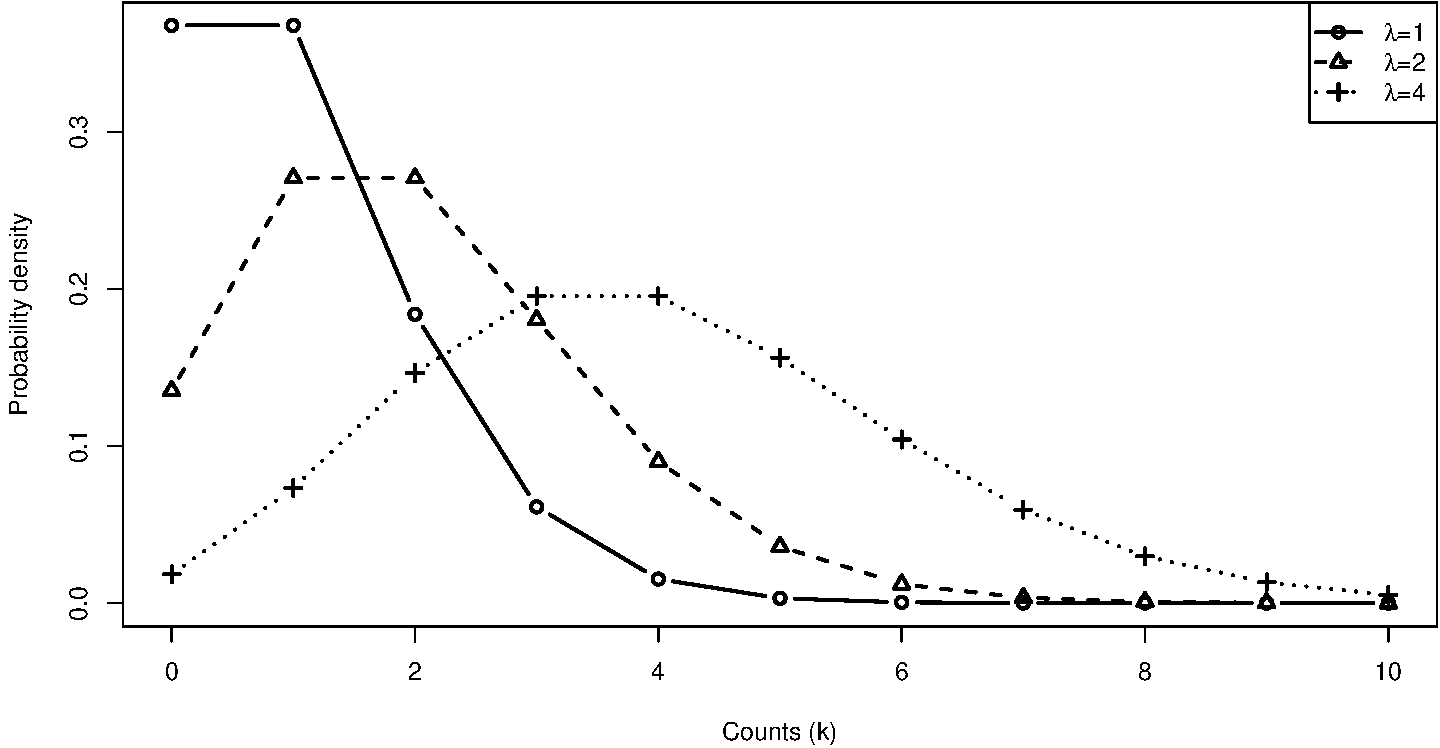
\includegraphics{../docs/articles/session_lecture_files/figure-beamer/unnamed-chunk-1-1.pdf}

\end{frame}

\begin{frame}{Poisson model: the GLM}
\protect\hypertarget{poisson-model-the-glm}{}

The \textbf{systematic part} of the GLM is: \[
log(\lambda_i) = \beta_0 + \beta_1 \textrm{RACE}_i + \beta_2 \textrm{TRT}_i + \beta_3 \textrm{ALCH}_i + \beta_4 \textrm{DRUG}_i
\] Or alternatively: \[
\lambda_i = exp \left( \beta_0 + \beta_1 \textrm{RACE}_i + \beta_2 \textrm{TRT}_i + \beta_3 \textrm{ALCH}_i + \beta_4 \textrm{DRUG}_i \right)
\]

The \textbf{random part} is (Recall the \(\lambda_i\) is both the mean
and variance of a Poisson distribution): \[
y_i \sim Poisson(\lambda_i)
\]

\end{frame}

\begin{frame}[fragile]{Example: Risky Drug Use Behavior}
\protect\hypertarget{example-risky-drug-use-behavior}{}

\begin{itemize}
\tightlist
\item
  Load the ``needle\_sharing'' dataset
\item
  Outcome is \# times the drug user shared a syringe in the past month
  (\texttt{shared\_syr})
\item
  Predictors: \texttt{sex}, \texttt{ethn}, \texttt{homeless}

  \begin{itemize}
  \tightlist
  \item
    filtered to only \texttt{sex} ``M'' or ``F'', \texttt{ethn}
    ``White'', ``AA'', ``Hispanic''
  \end{itemize}
\end{itemize}

\small

\begin{Shaded}
\begin{Highlighting}[]
\KeywordTok{summary}\NormalTok{(needledat2}\OperatorTok{$}\NormalTok{shared_syr)}
\end{Highlighting}
\end{Shaded}

\begin{verbatim}
##    Min. 1st Qu.  Median    Mean 3rd Qu.    Max.    NA's 
##   0.000   0.000   0.000   3.122   0.000  60.000       2
\end{verbatim}

\begin{Shaded}
\begin{Highlighting}[]
\KeywordTok{var}\NormalTok{(needledat2}\OperatorTok{$}\NormalTok{shared_syr, }\DataTypeTok{na.rm =} \OtherTok{TRUE}\NormalTok{)}
\end{Highlighting}
\end{Shaded}

\begin{verbatim}
## [1] 113.371
\end{verbatim}

\end{frame}

\begin{frame}{Example: Risky Drug Use Behavior}
\protect\hypertarget{example-risky-drug-use-behavior-1}{}

Exploratory plots

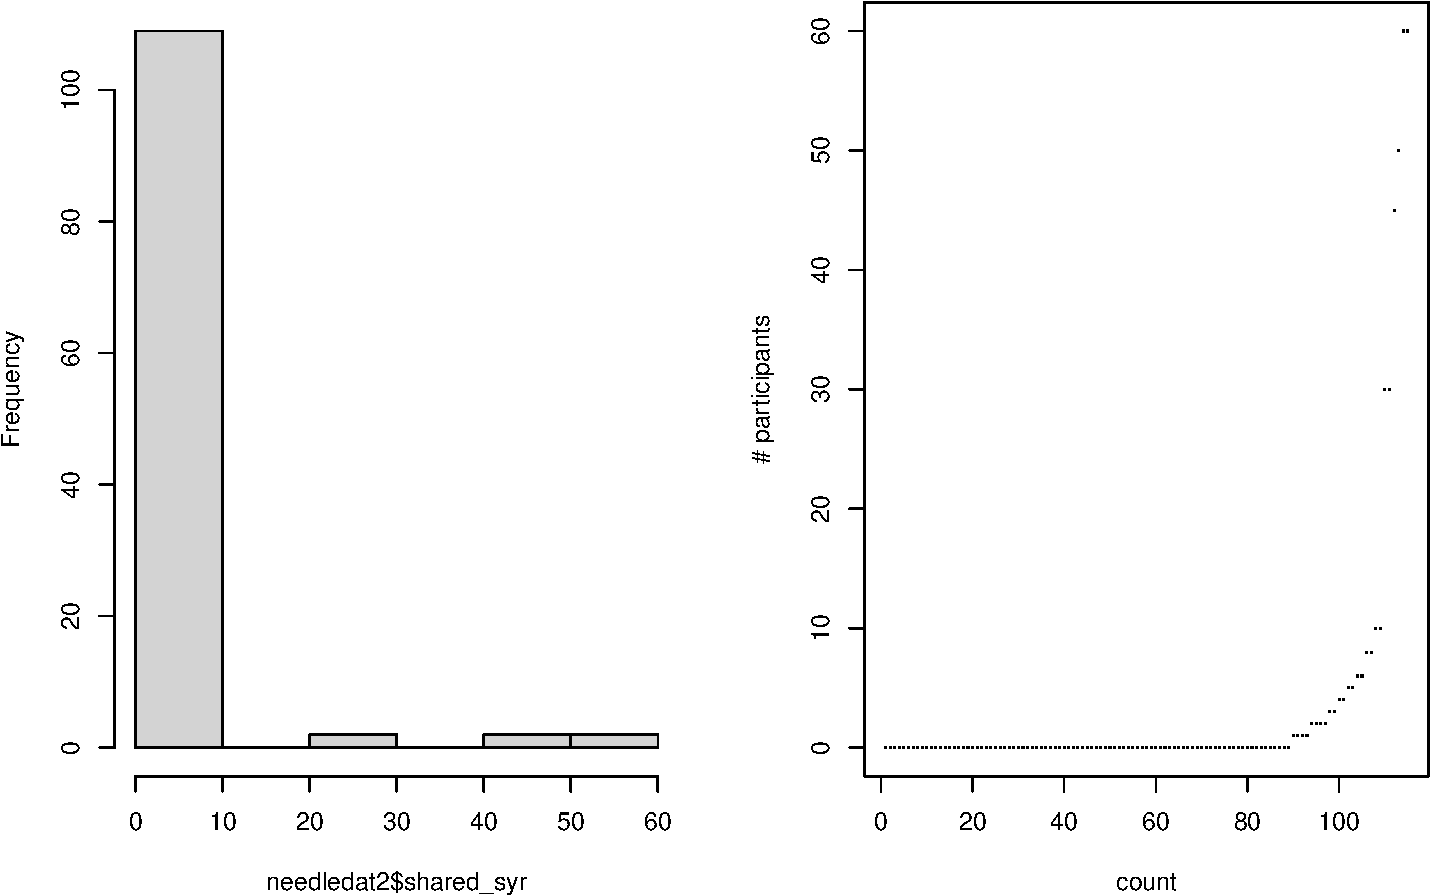
\includegraphics{../docs/articles/session_lecture_files/figure-beamer/unnamed-chunk-3-1.pdf}

\begin{itemize}
\tightlist
\item
  There are a \emph{lot} of zeros and variance is much greater than mean

  \begin{itemize}
  \tightlist
  \item
    Poisson model is probably not a good fit
  \end{itemize}
\end{itemize}

\end{frame}

\begin{frame}[fragile]{Risky Drug Use Behavior: fitting a Poisson model}
\protect\hypertarget{risky-drug-use-behavior-fitting-a-poisson-model}{}

\begin{Shaded}
\begin{Highlighting}[]
\NormalTok{fit.pois <-}\StringTok{ }\KeywordTok{glm}\NormalTok{(shared_syr }\OperatorTok{~}\StringTok{ }\NormalTok{sex }\OperatorTok{+}\StringTok{ }\NormalTok{ethn }\OperatorTok{+}\StringTok{ }\NormalTok{homeless,}
                \DataTypeTok{data =}\NormalTok{ needledat2,}
                \DataTypeTok{family =} \KeywordTok{poisson}\NormalTok{(}\DataTypeTok{link =} \StringTok{"log"}\NormalTok{))}
\end{Highlighting}
\end{Shaded}

\end{frame}

\begin{frame}{Risky Drug Use Behavior: residuals plots}
\protect\hypertarget{risky-drug-use-behavior-residuals-plots}{}

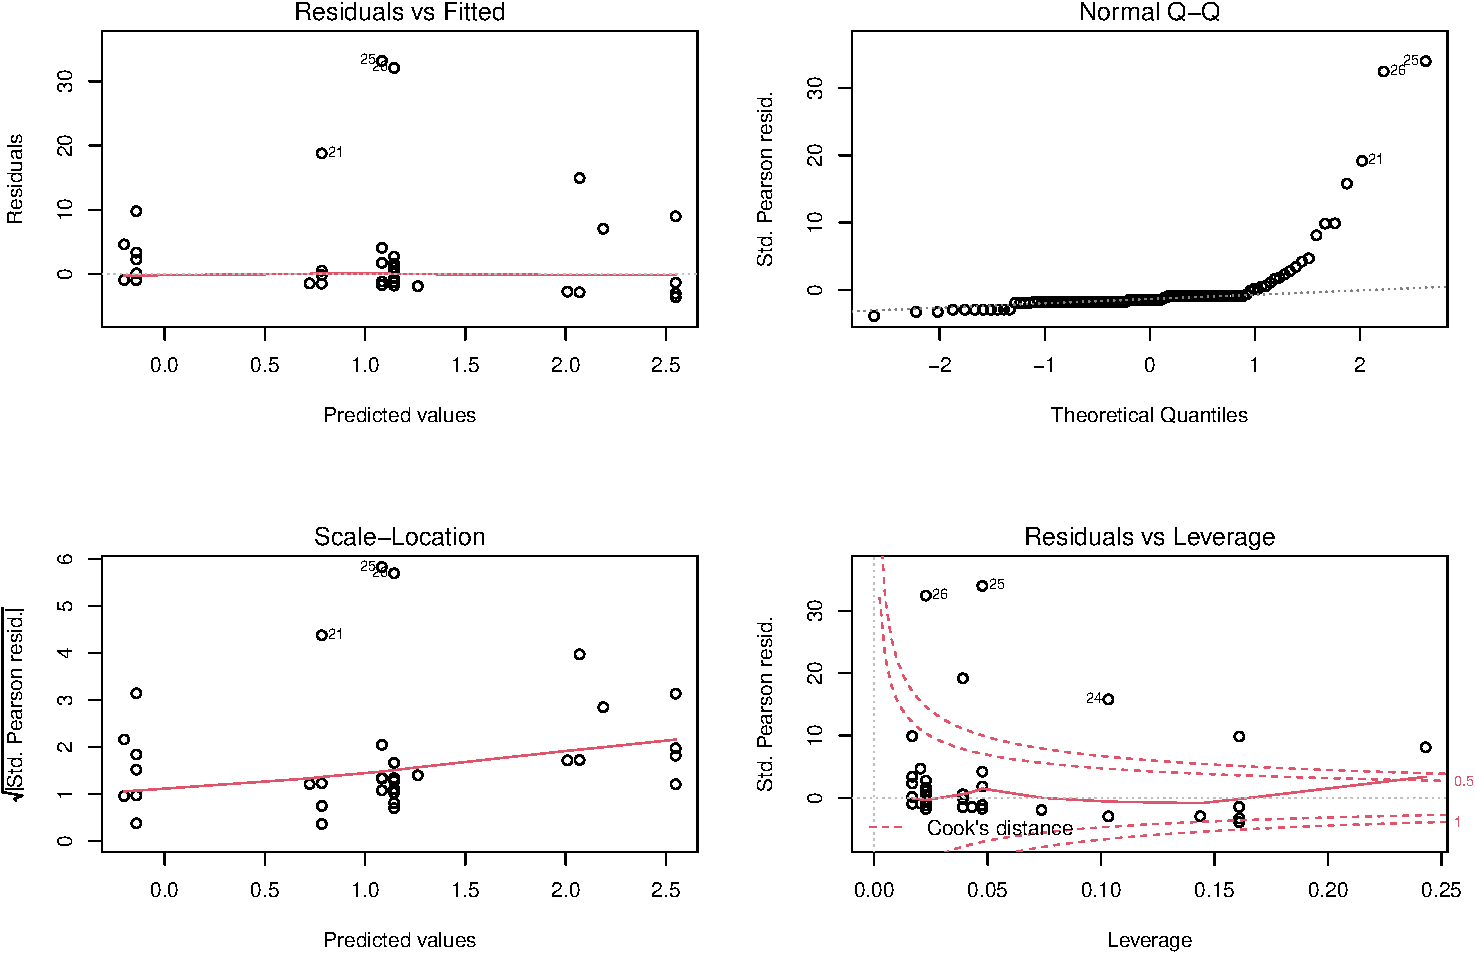
\includegraphics{../docs/articles/session_lecture_files/figure-beamer/unnamed-chunk-5-1.pdf}
* Poisson model is definitely not a good fit.

\end{frame}

\hypertarget{over-dispersion}{%
\section{Over-dispersion}\label{over-dispersion}}

\begin{frame}{When the Poisson model doesn't fit}
\protect\hypertarget{when-the-poisson-model-doesnt-fit}{}

\begin{itemize}
\tightlist
\item
  inference from log-linear models is sensitive to assumptions on the
  distribution of residuals (e.g.~Poisson)
\item
  In the Poisson distribution, the variance is equal to the mean.
\item
  \emph{i.e.} if subjects with a particular pattern of covariates have a
  mean of 4 visits/yr, then variance is also 4 and the standard
  deviation is 2 visits / yr.
\item
  The Poisson distribution often fails when the variance exceeds the
  mean

  \begin{itemize}
  \tightlist
  \item
    You can \emph{check} this assumption\\
  \end{itemize}
\item
  Can use alternative random distributions:

  \begin{itemize}
  \tightlist
  \item
    Negative binomial distribution
  \end{itemize}
\item
  Can introduce zero-inflation
\end{itemize}

\end{frame}

\begin{frame}{Negative binomial distribution}
\protect\hypertarget{negative-binomial-distribution}{}

\begin{itemize}
\tightlist
\item
  The binomial distribution is the number of successes in n trials:

  \begin{itemize}
  \tightlist
  \item
    Roll a die ten times, how many times do you see a 6?
  \end{itemize}
\item
  The negative binomial distribution is the number of successes it takes
  to observe r failures:

  \begin{itemize}
  \tightlist
  \item
    How many times do you have to roll the die to see a 6 ten times?
  \item
    Note that the number of rolls is no longer fixed.
  \item
    In this example, p=5/6 and a 6 is a ``failure''
  \end{itemize}
\end{itemize}

\end{frame}

\begin{frame}[fragile]{Negative binomial GLM}
\protect\hypertarget{negative-binomial-glm}{}

\emph{One way} to parametrize a NB model is with a \textbf{systematic
part} equivalent to the Poisson model: \[
log(\lambda_i) = \beta_0 + \beta_1 \textrm{RACE}_i + \beta_2 \textrm{TRT}_i + \beta_3 \textrm{ALCH}_i + \beta_4 \textrm{DRUG}_i
\] Or: \[
\lambda_i = exp \left( \beta_0 + \beta_1 \textrm{RACE}_i + \beta_2 \textrm{TRT}_i + \beta_3 \textrm{ALCH}_i + \beta_4 \textrm{DRUG}_i \right)
\]

And a \textbf{random part}: \[
y_i \sim NB(\lambda_i, \theta)
\]

\begin{itemize}
\tightlist
\item
  \(\theta\) is a \textbf{dispersion parameter} that is estimated
\item
  When \(\theta = 0\) it is equivalent to Poisson model
\item
  \texttt{MASS::glm.nb()} uses this parametrization, \texttt{dnbinom()}
  does not
\item
  The Poisson model can be considered \textbf{nested} within the
  Negative Binomial model
\end{itemize}

\end{frame}

\begin{frame}{Negative Binomial Random Distribution}
\protect\hypertarget{negative-binomial-random-distribution}{}

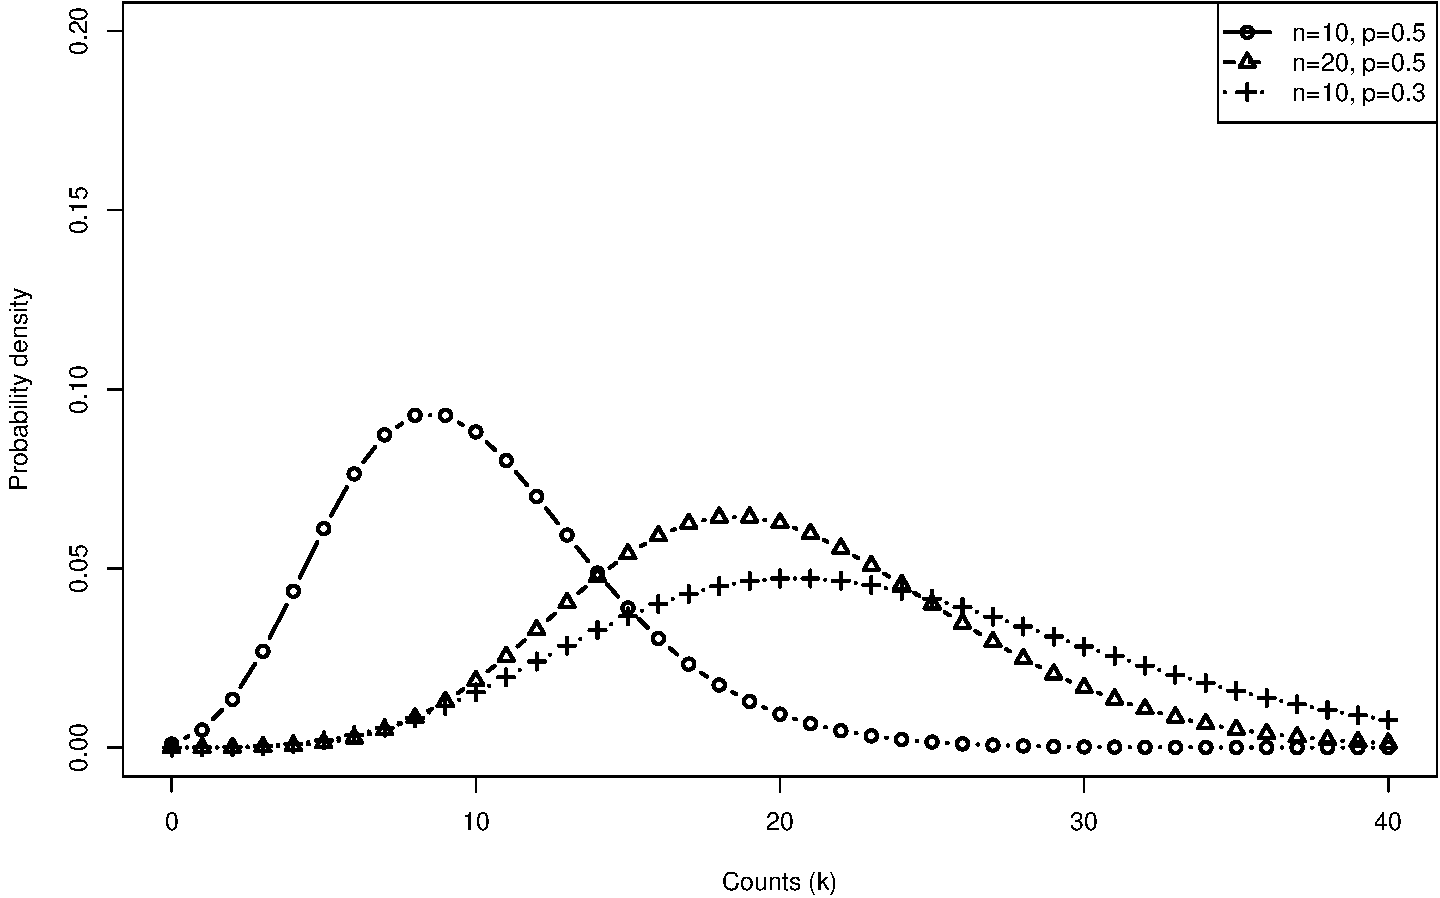
\includegraphics{../docs/articles/session_lecture_files/figure-beamer/unnamed-chunk-6-1.pdf}

\end{frame}

\begin{frame}{Compare Poisson vs.~Negative Binomial}
\protect\hypertarget{compare-poisson-vs.-negative-binomial}{}

Negative Binomial Distribution has two parameters: \# of trials n, and
probability of success p

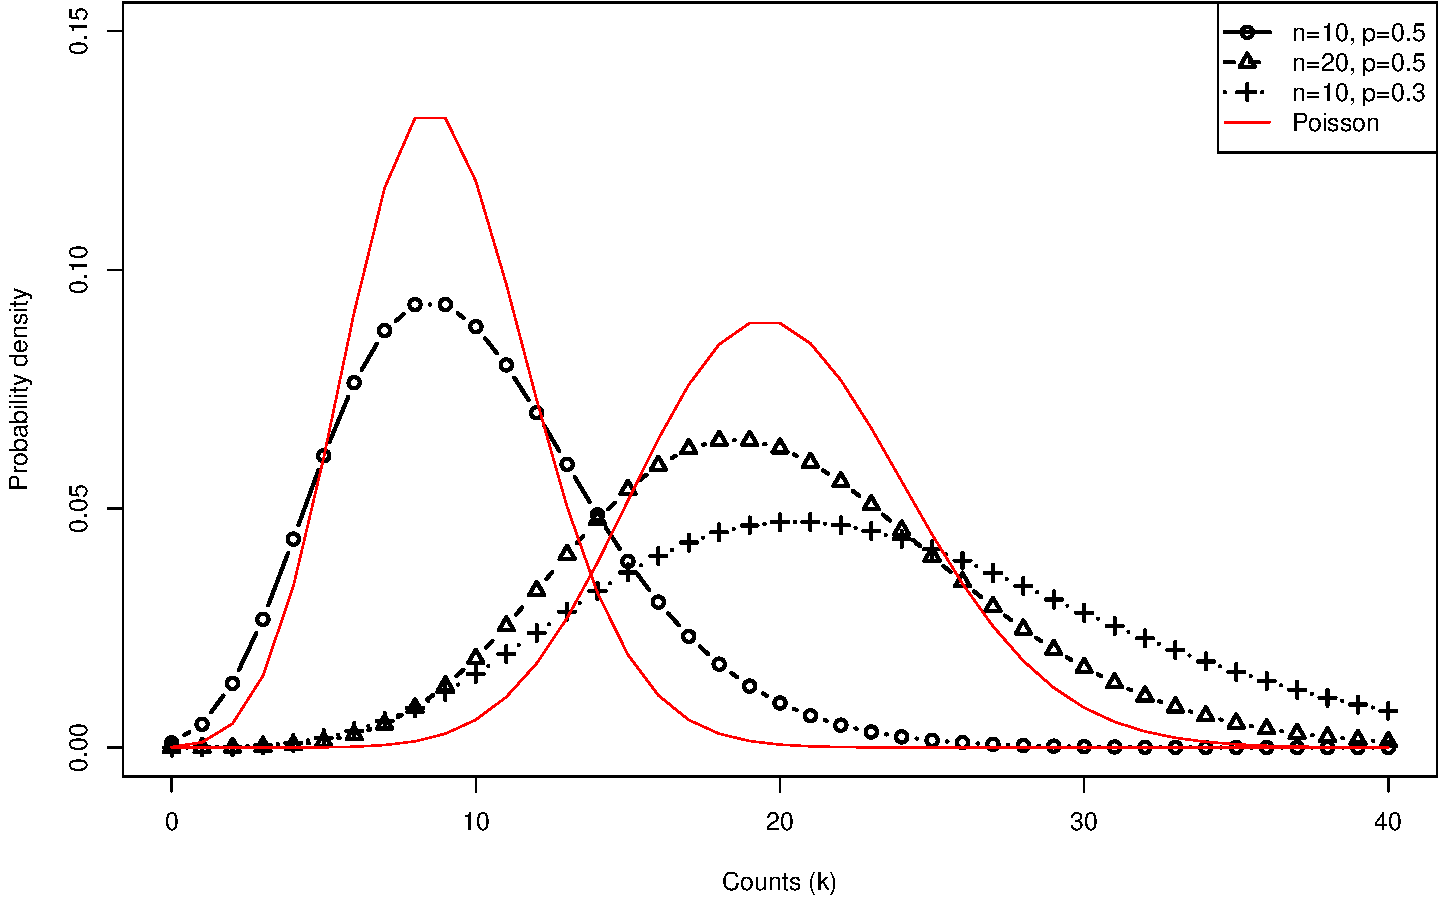
\includegraphics{../docs/articles/session_lecture_files/figure-beamer/unnamed-chunk-7-1.pdf}

\end{frame}

\begin{frame}[fragile]{Risky drug behavior: Negative Binomial
Regression}
\protect\hypertarget{risky-drug-behavior-negative-binomial-regression}{}

\begin{Shaded}
\begin{Highlighting}[]
\KeywordTok{library}\NormalTok{(MASS)}
\NormalTok{fit.negbin <-}\StringTok{ }\NormalTok{MASS}\OperatorTok{::}\KeywordTok{glm.nb}\NormalTok{(shared_syr }\OperatorTok{~}\StringTok{ }\NormalTok{sex }\OperatorTok{+}
\StringTok{                             }\NormalTok{ethn }\OperatorTok{+}\StringTok{ }\NormalTok{homeless,}
                           \DataTypeTok{data =}\NormalTok{ needledat2)}
\end{Highlighting}
\end{Shaded}

\end{frame}

\begin{frame}[fragile]{}
\protect\hypertarget{section}{}

\tiny

\begin{Shaded}
\begin{Highlighting}[]
\KeywordTok{summary}\NormalTok{(fit.negbin)}
\end{Highlighting}
\end{Shaded}

\begin{verbatim}
## 
## Call:
## MASS::glm.nb(formula = shared_syr ~ sex + ethn + homeless, data = needledat2, 
##     init.theta = 0.07743871374, link = log)
## 
## Deviance Residuals: 
##     Min       1Q   Median       3Q      Max  
## -0.8801  -0.7787  -0.6895  -0.5748   1.5675  
## 
## Coefficients:
##              Estimate Std. Error z value Pr(>|z|)  
## (Intercept)    0.4641     0.8559   0.542   0.5876  
## sexM          -1.0148     0.8294  -1.224   0.2211  
## ethnHispanic   1.3424     1.3201   1.017   0.3092  
## ethnWhite      0.2429     0.7765   0.313   0.7544  
## homelessyes    1.6445     0.7073   2.325   0.0201 *
## ---
## Signif. codes:  0 '***' 0.001 '**' 0.01 '*' 0.05 '.' 0.1 ' ' 1
## 
## (Dispersion parameter for Negative Binomial(0.0774) family taken to be 1)
## 
##     Null deviance: 62.365  on 114  degrees of freedom
## Residual deviance: 56.232  on 110  degrees of freedom
##   (2 observations deleted due to missingness)
## AIC: 306.26
## 
## Number of Fisher Scoring iterations: 1
## 
## 
##               Theta:  0.0774 
##           Std. Err.:  0.0184 
## 
##  2 x log-likelihood:  -294.2550
\end{verbatim}

\end{frame}

\begin{frame}[fragile]{Likelihood ratio test}
\protect\hypertarget{likelihood-ratio-test}{}

Basis: Under \(H_0\): no improvement in fit by more complex model,
difference in model residual deviances is \(\chi^2\)-distributed.

Deviance:
\(\Delta (\textrm{D}) = -2 * \Delta (\textrm{log likelihood})\)

\begin{Shaded}
\begin{Highlighting}[]
\NormalTok{(ll.negbin <-}\StringTok{ }\KeywordTok{logLik}\NormalTok{(fit.negbin))}
\end{Highlighting}
\end{Shaded}

\begin{verbatim}
## 'log Lik.' -147.1277 (df=6)
\end{verbatim}

\begin{Shaded}
\begin{Highlighting}[]
\NormalTok{(ll.pois <-}\StringTok{ }\KeywordTok{logLik}\NormalTok{(fit.pois))}
\end{Highlighting}
\end{Shaded}

\begin{verbatim}
## 'log Lik.' -730.0133 (df=5)
\end{verbatim}

\begin{Shaded}
\begin{Highlighting}[]
\KeywordTok{pchisq}\NormalTok{(}\DecValTok{2} \OperatorTok{*}\StringTok{ }\NormalTok{(ll.negbin }\OperatorTok{-}\StringTok{ }\NormalTok{ll.pois), }\DataTypeTok{df=}\DecValTok{1}\NormalTok{, }
       \DataTypeTok{lower.tail=}\OtherTok{FALSE}\NormalTok{)}
\end{Highlighting}
\end{Shaded}

\begin{verbatim}
## 'log Lik.' 1.675949e-255 (df=6)
\end{verbatim}

\end{frame}

\begin{frame}{NB regression residuals plots}
\protect\hypertarget{nb-regression-residuals-plots}{}

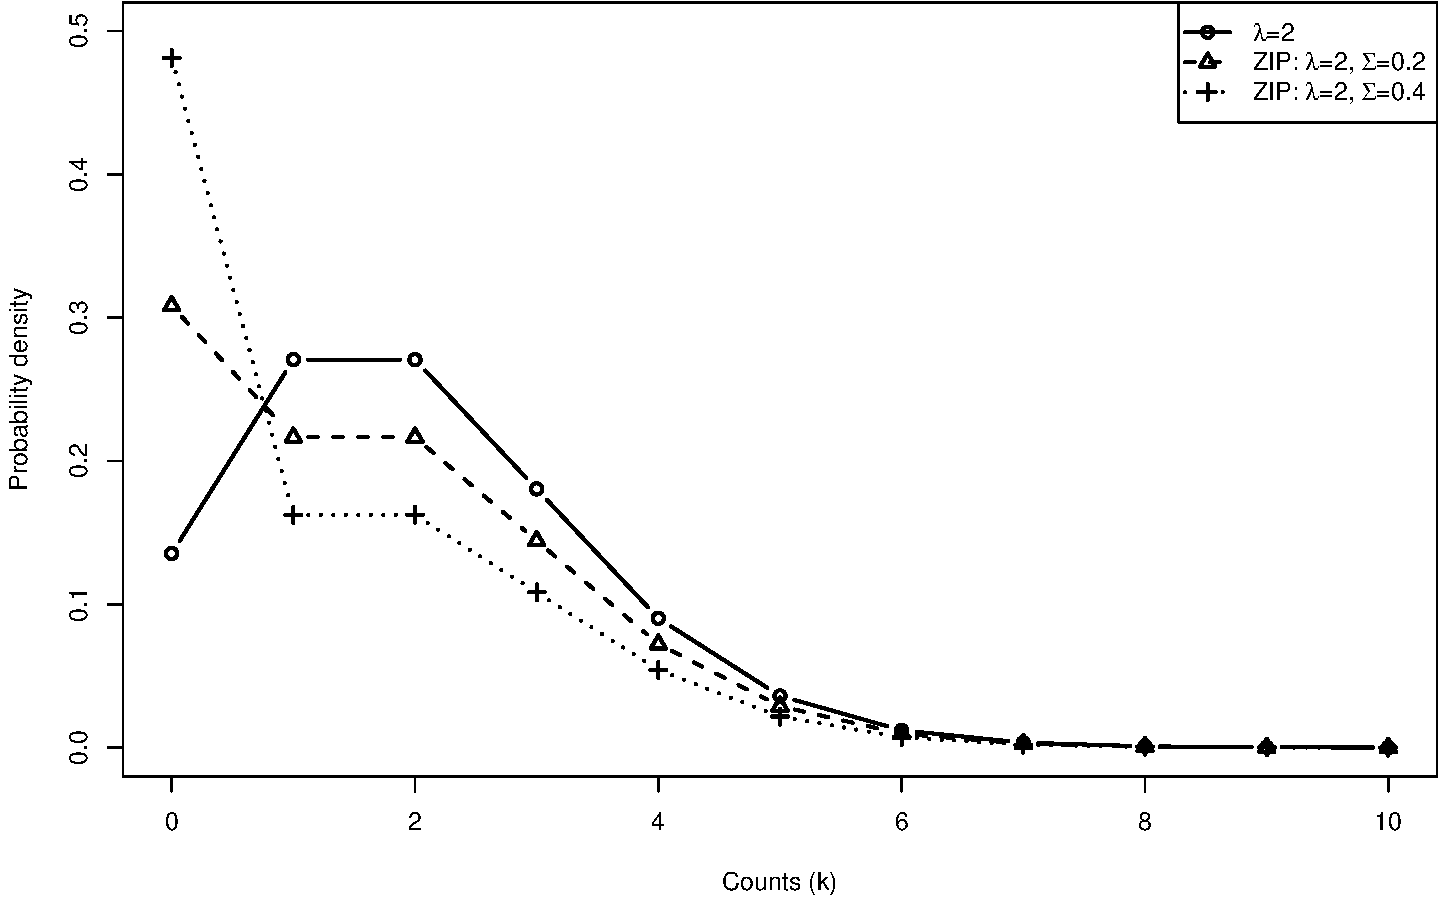
\includegraphics{../docs/articles/session_lecture_files/figure-beamer/unnamed-chunk-11-1.pdf}

\end{frame}

\hypertarget{zero-inflation}{%
\section{Zero Inflation}\label{zero-inflation}}

\begin{frame}{Zero inflated ``two-step'' models}
\protect\hypertarget{zero-inflated-two-step-models}{}

\textbf{Step 1}: logistic model to determine whether count is zero or
Poisson/NB

\textbf{Step 2}: Poisson or NB regression distribution for \(y_i\) not
set to zero by \emph{1.}

\end{frame}

\begin{frame}{Poisson Distribution with Zero Inflation}
\protect\hypertarget{poisson-distribution-with-zero-inflation}{}

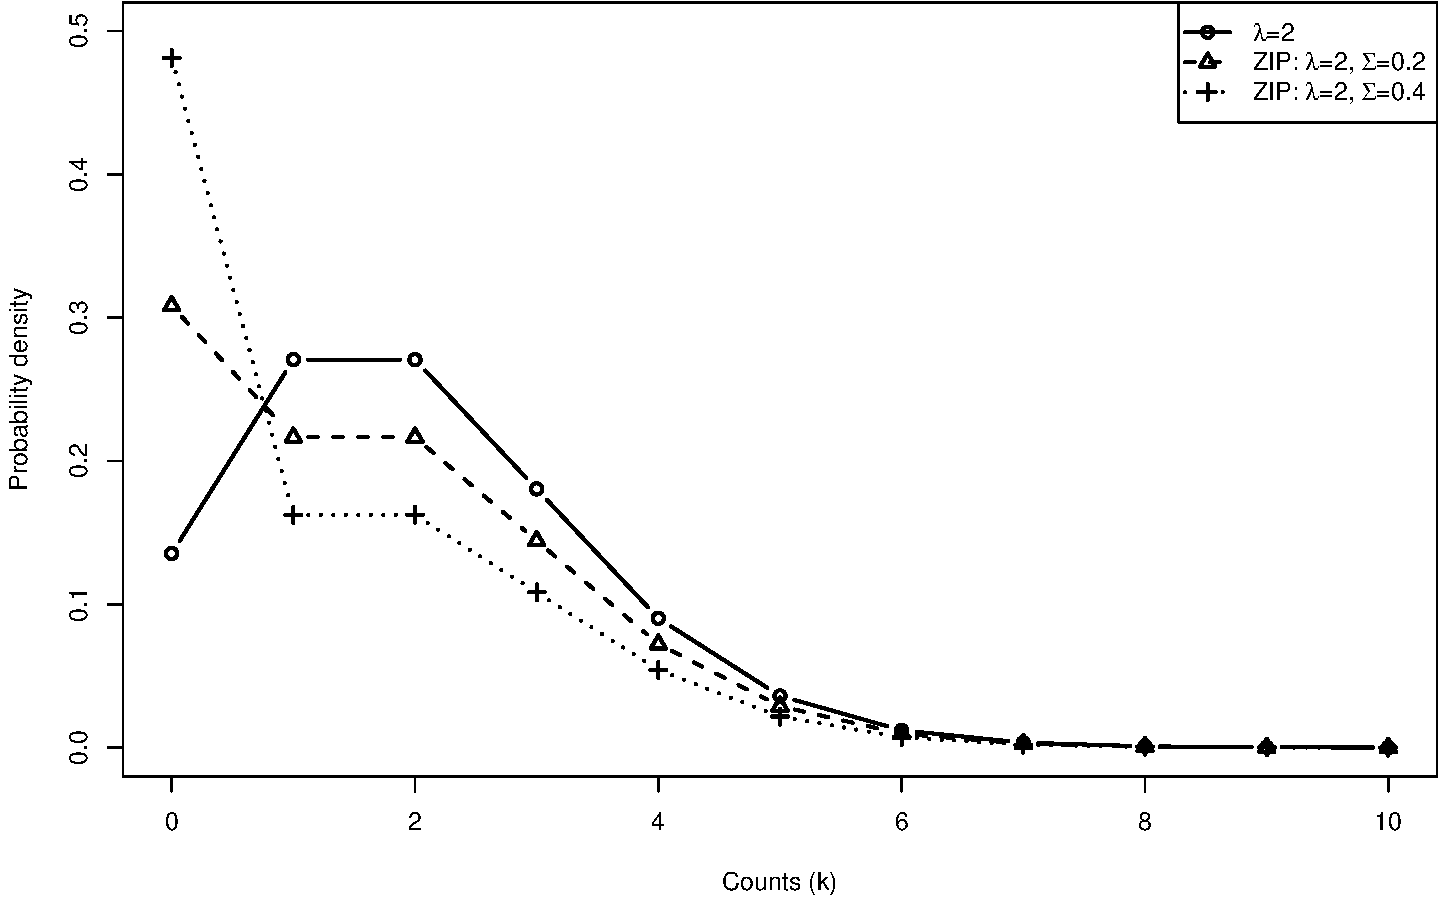
\includegraphics{../docs/articles/session_lecture_files/figure-beamer/unnamed-chunk-12-1.pdf}

\end{frame}

\begin{frame}[fragile]{Risky drug behavior: Zero-inflated Poisson
regression}
\protect\hypertarget{risky-drug-behavior-zero-inflated-poisson-regression}{}

\begin{Shaded}
\begin{Highlighting}[]
\KeywordTok{library}\NormalTok{(pscl)}
\NormalTok{fit.ZIpois <-}\StringTok{ }\KeywordTok{zeroinfl}\NormalTok{(shared_syr }\OperatorTok{~}\StringTok{ }\NormalTok{sex }\OperatorTok{+}\StringTok{ }\NormalTok{ethn }\OperatorTok{+}\StringTok{ }\NormalTok{homeless,}
                       \DataTypeTok{dist =} \StringTok{"poisson"}\NormalTok{,}
                       \DataTypeTok{data =}\NormalTok{ needledat2)}
\end{Highlighting}
\end{Shaded}

\end{frame}

\begin{frame}[fragile]{Zero-inflated Poisson regression - the model}
\protect\hypertarget{zero-inflated-poisson-regression---the-model}{}

\begin{Shaded}
\begin{Highlighting}[]
\KeywordTok{summary}\NormalTok{(fit.ZIpois)}
\end{Highlighting}
\end{Shaded}

\begin{verbatim}
## 
## Call:
## zeroinfl(formula = shared_syr ~ sex + ethn + homeless, data = needledat2, 
##     dist = "poisson")
## 
## Pearson residuals:
##     Min      1Q  Median      3Q     Max 
## -1.0761 -0.5784 -0.4030 -0.3341 10.6835 
## 
## Count model coefficients (poisson with log link):
##              Estimate Std. Error z value Pr(>|z|)    
## (Intercept)    3.2168     0.1796  17.908  < 2e-16 ***
## sexM          -1.4725     0.1442 -10.212  < 2e-16 ***
## ethnHispanic  -0.1524     0.1576  -0.968 0.333244    
## ethnWhite     -0.5236     0.1464  -3.577 0.000348 ***
## homelessyes    1.2034     0.1455   8.268  < 2e-16 ***
## 
## Zero-inflation model coefficients (binomial with logit link):
##              Estimate Std. Error z value Pr(>|z|)   
## (Intercept)   2.06263    0.65227   3.162  0.00157 **
## sexM         -0.05068    0.58252  -0.087  0.93068   
## ethnHispanic -1.76122    0.81177  -2.170  0.03004 * 
## ethnWhite    -0.50187    0.56919  -0.882  0.37792   
## homelessyes  -0.53013    0.48108  -1.102  0.27047   
## ---
## Signif. codes:  0 '***' 0.001 '**' 0.01 '*' 0.05 '.' 0.1 ' ' 1 
## 
## Number of iterations in BFGS optimization: 12 
## Log-likelihood: -299.8 on 10 Df
\end{verbatim}

\end{frame}

\begin{frame}[fragile]{Risky drug behavior: Zero-inflated Negative
Binomial regression}
\protect\hypertarget{risky-drug-behavior-zero-inflated-negative-binomial-regression}{}

\begin{Shaded}
\begin{Highlighting}[]
\NormalTok{fit.ZInegbin <-}\StringTok{ }\KeywordTok{zeroinfl}\NormalTok{(shared_syr }\OperatorTok{~}\StringTok{ }\NormalTok{sex }\OperatorTok{+}\StringTok{ }\NormalTok{ethn }\OperatorTok{+}\StringTok{ }\NormalTok{homeless,}
                         \DataTypeTok{dist =} \StringTok{"negbin"}\NormalTok{,}
                         \DataTypeTok{data =}\NormalTok{ needledat2)}
\end{Highlighting}
\end{Shaded}

\begin{itemize}
\tightlist
\item
  \emph{NOTE}: zero-inflation model can include any of your variables as
  predictors
\item
  \emph{WARNING} Default in \texttt{zerinfl()} function is to use
  \emph{all} variables as predictors in logistic model
\end{itemize}

\end{frame}

\begin{frame}[fragile]{Zero-inflated Negative Binomial regression -
model 1}
\protect\hypertarget{zero-inflated-negative-binomial-regression---model-1}{}

\tiny

\begin{Shaded}
\begin{Highlighting}[]
\KeywordTok{summary}\NormalTok{(fit.ZInegbin)}
\end{Highlighting}
\end{Shaded}

\begin{verbatim}
## 
## Call:
## zeroinfl(formula = shared_syr ~ sex + ethn + homeless, data = needledat2, 
##     dist = "negbin")
## 
## Pearson residuals:
##     Min      1Q  Median      3Q     Max 
## -0.5402 -0.3255 -0.2714 -0.1926  5.1496 
## 
## Count model coefficients (negbin with log link):
##              Estimate Std. Error z value Pr(>|z|)   
## (Intercept)    2.8410     1.1845   2.399  0.01646 * 
## sexM          -2.2282     0.9351  -2.383  0.01718 * 
## ethnHispanic  -0.4123     0.9831  -0.419  0.67492   
## ethnWhite     -0.4299     0.8648  -0.497  0.61908   
## homelessyes    1.9460     0.7103   2.740  0.00615 **
## Log(theta)    -1.1971     0.5159  -2.320  0.02032 * 
## 
## Zero-inflation model coefficients (binomial with logit link):
##              Estimate Std. Error z value Pr(>|z|)  
## (Intercept)    1.6867     0.8465   1.993   0.0463 *
## sexM          -0.9920     0.8016  -1.238   0.2159  
## ethnHispanic -13.1868   281.9134  -0.047   0.9627  
## ethnWhite     -0.7455     0.7304  -1.021   0.3074  
## homelessyes    0.3554     0.7397   0.480   0.6309  
## ---
## Signif. codes:  0 '***' 0.001 '**' 0.01 '*' 0.05 '.' 0.1 ' ' 1 
## 
## Theta = 0.3021 
## Number of iterations in BFGS optimization: 24 
## Log-likelihood: -142.8 on 11 Df
\end{verbatim}

\end{frame}

\begin{frame}[fragile]{Zero-inflated Negative Binomial regression -
simplified ZI model}
\protect\hypertarget{zero-inflated-negative-binomial-regression---simplified-zi-model}{}

\begin{itemize}
\tightlist
\item
  Model is much more interpretable if the exposure of interest is
  \emph{not} included in the zero-inflation model.
\item
  E.g. with HIV status as the only predictor in zero-inflation model:
\end{itemize}

\begin{Shaded}
\begin{Highlighting}[]
\NormalTok{fit.ZInb2 <-}\StringTok{ }\KeywordTok{zeroinfl}\NormalTok{(shared_syr }\OperatorTok{~}\StringTok{ }\NormalTok{sex }\OperatorTok{+}\StringTok{ }\NormalTok{ethn }\OperatorTok{+}\StringTok{ }\NormalTok{homeless }\OperatorTok{+}\StringTok{ }\NormalTok{hiv }\OperatorTok{|}\StringTok{ }\NormalTok{hiv,}
                      \DataTypeTok{dist =} \StringTok{"negbin"}\NormalTok{,}
                      \DataTypeTok{data =}\NormalTok{ needledat2)}
\end{Highlighting}
\end{Shaded}

\end{frame}

\begin{frame}[fragile]{Zero-inflated Negative Binomial regression -
model 2}
\protect\hypertarget{zero-inflated-negative-binomial-regression---model-2}{}

\tiny

\begin{Shaded}
\begin{Highlighting}[]
\KeywordTok{summary}\NormalTok{(fit.ZInb2)}
\end{Highlighting}
\end{Shaded}

\begin{verbatim}
## 
## Call:
## zeroinfl(formula = shared_syr ~ sex + ethn + homeless + hiv | hiv, data = needledat2, 
##     dist = "negbin")
## 
## Pearson residuals:
##     Min      1Q  Median      3Q     Max 
## -0.4299 -0.3646 -0.3559 -0.3299  6.3053 
## 
## Count model coefficients (negbin with log link):
##              Estimate Std. Error z value Pr(>|z|)    
## (Intercept)    3.6685     0.9470   3.874 0.000107 ***
## sexM          -1.7648     0.6205  -2.844 0.004454 ** 
## ethnHispanic  -1.5807     0.7446  -2.123 0.033769 *  
## ethnWhite     -1.1267     0.6924  -1.627 0.103687    
## homelessyes    1.0313     0.5693   1.812 0.070028 .  
## hivpositive   -1.0820     1.0167  -1.064 0.287235    
## hivyes         2.3724     0.7829   3.030 0.002444 ** 
## Log(theta)     0.1395     0.4647   0.300 0.764009    
## 
## Zero-inflation model coefficients (binomial with logit link):
##              Estimate Std. Error z value Pr(>|z|)    
## (Intercept)    1.2163     0.2851   4.265    2e-05 ***
## hivpositive   -0.3493     0.9389  -0.372    0.710    
## hivyes       -17.9654  3065.6271  -0.006    0.995    
## ---
## Signif. codes:  0 '***' 0.001 '**' 0.01 '*' 0.05 '.' 0.1 ' ' 1 
## 
## Theta = 1.1497 
## Number of iterations in BFGS optimization: 12 
## Log-likelihood: -122.5 on 11 Df
\end{verbatim}

\end{frame}

\begin{frame}[fragile]{Intercept-only zero-inflation model}
\protect\hypertarget{intercept-only-zero-inflation-model}{}

\tiny

\begin{Shaded}
\begin{Highlighting}[]
\NormalTok{fit.ZInb3 <-}\StringTok{ }\KeywordTok{zeroinfl}\NormalTok{(shared_syr}\OperatorTok{~}\NormalTok{sex}\OperatorTok{+}\NormalTok{ethn}\OperatorTok{+}\NormalTok{homeless}\OperatorTok{|}\DecValTok{1}\NormalTok{, }
                        \DataTypeTok{dist=}\StringTok{"negbin"}\NormalTok{, }\DataTypeTok{data=}\NormalTok{needledat2)}
\KeywordTok{summary}\NormalTok{(fit.ZInb3)}
\end{Highlighting}
\end{Shaded}

\begin{verbatim}
## 
## Call:
## zeroinfl(formula = shared_syr ~ sex + ethn + homeless | 1, data = needledat2, 
##     dist = "negbin")
## 
## Pearson residuals:
##     Min      1Q  Median      3Q     Max 
## -0.3159 -0.3123 -0.3040 -0.2953  5.2940 
## 
## Count model coefficients (negbin with log link):
##              Estimate Std. Error z value Pr(>|z|)  
## (Intercept)   2.08542    1.42671   1.462   0.1438  
## sexM         -1.43809    0.89189  -1.612   0.1069  
## ethnHispanic  0.48130    1.16642   0.413   0.6799  
## ethnWhite    -0.07418    0.81066  -0.092   0.9271  
## homelessyes   1.62076    0.67706   2.394   0.0167 *
## Log(theta)   -1.12538    0.89372  -1.259   0.2080  
## 
## Zero-inflation model coefficients (binomial with logit link):
##             Estimate Std. Error z value Pr(>|z|)
## (Intercept)   0.5211     0.7600   0.686    0.493
## ---
## Signif. codes:  0 '***' 0.001 '**' 0.01 '*' 0.05 '.' 0.1 ' ' 1 
## 
## Theta = 0.3245 
## Number of iterations in BFGS optimization: 13 
## Log-likelihood: -146.8 on 7 Df
\end{verbatim}

\end{frame}

\begin{frame}[fragile]{Residuals vs.~fitted values}
\protect\hypertarget{residuals-vs.-fitted-values}{}

I invisibly define functions \texttt{plotpanel1} and \texttt{plotpanel2}
that will work for all types of models (see lab). These use Pearson
residuals.

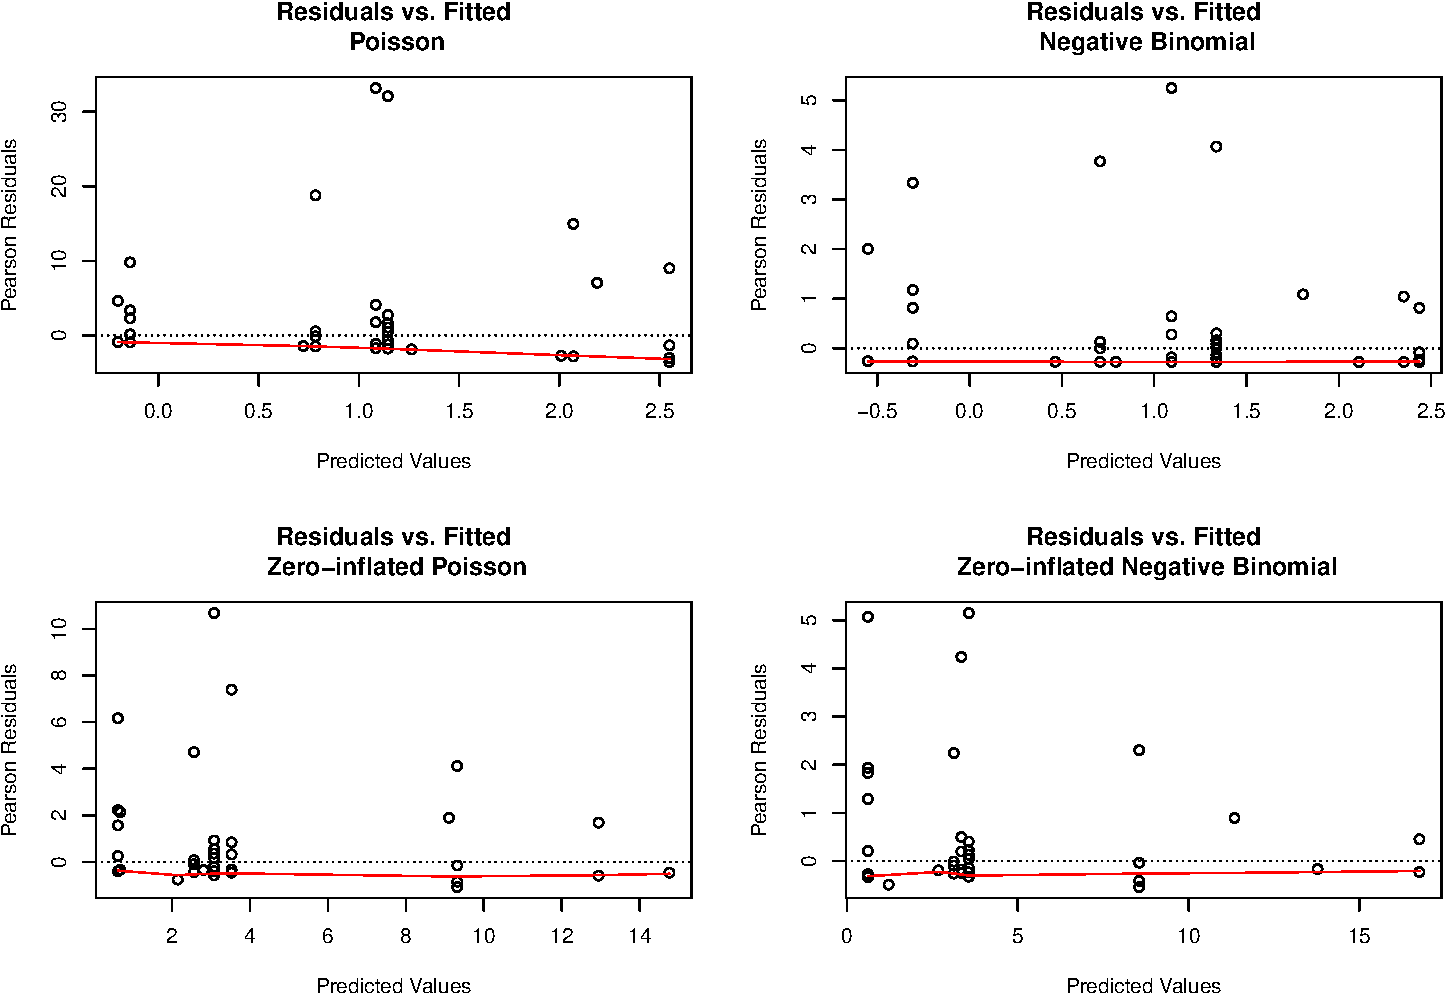
\includegraphics{../docs/articles/session_lecture_files/figure-beamer/unnamed-chunk-21-1.pdf}

\end{frame}

\begin{frame}{Quantile-quantile plots for residuals}
\protect\hypertarget{quantile-quantile-plots-for-residuals}{}

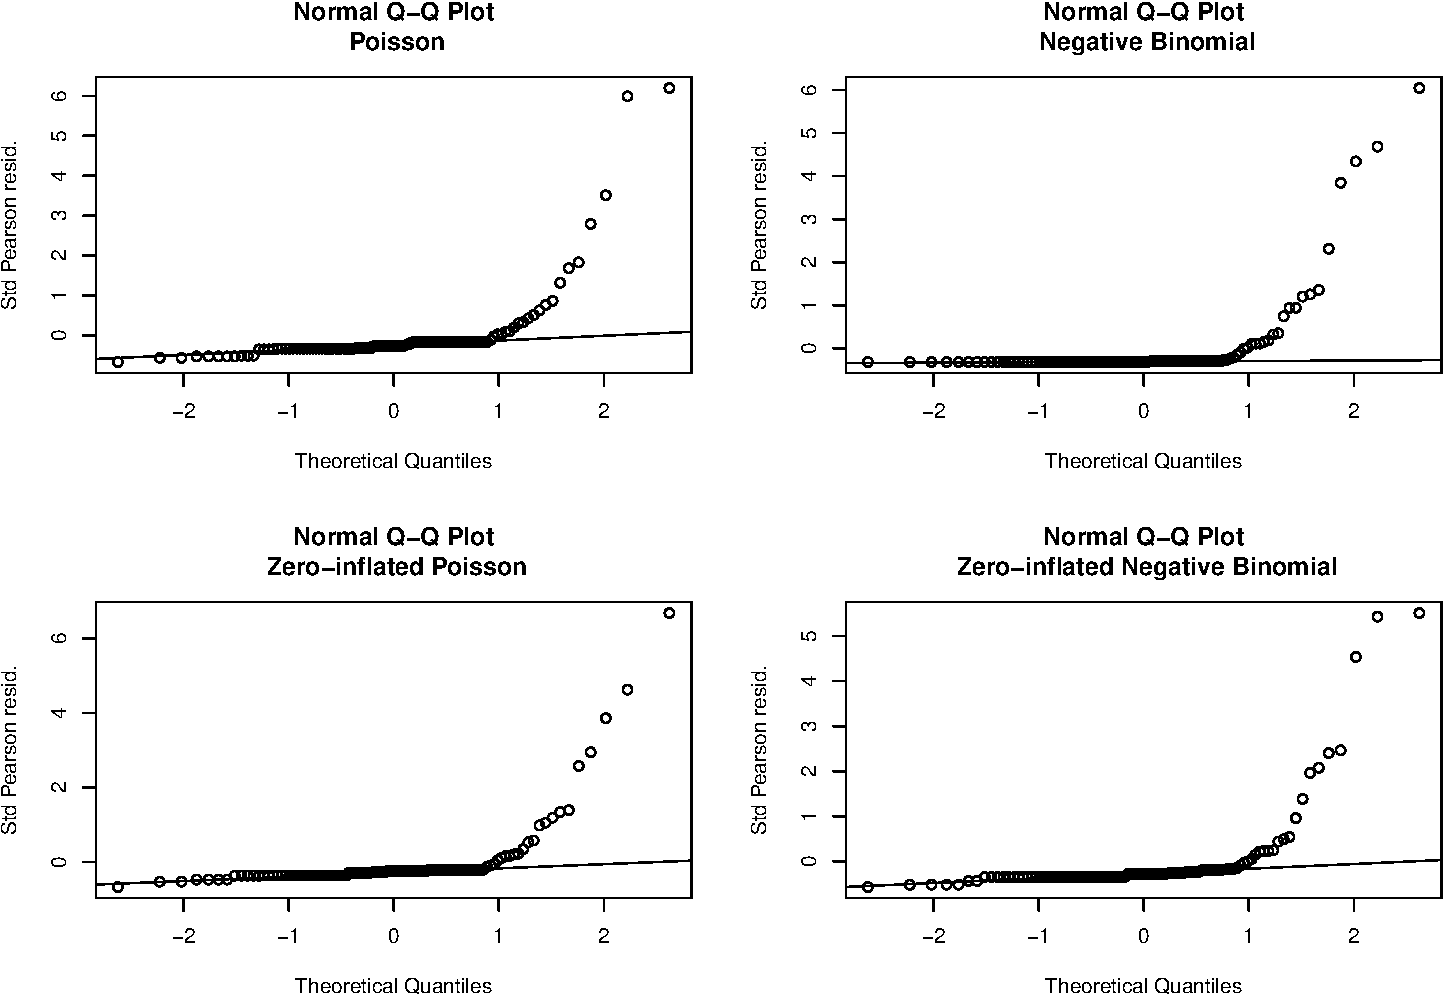
\includegraphics{../docs/articles/session_lecture_files/figure-beamer/unnamed-chunk-22-1.pdf}
\emph{still} over-dispersed - ideas?

\end{frame}

\begin{frame}{Inference from the different models}
\protect\hypertarget{inference-from-the-different-models}{}

\tiny

\% Error: Unrecognized object type. Zero-inflated models are 3) Poisson,
4) Negative Binomial, and 5) Negative Binomial with intercept-only zero
inflation model.

\end{frame}

\begin{frame}{Example of plotting observed and predicted counts}
\protect\hypertarget{example-of-plotting-observed-and-predicted-counts}{}

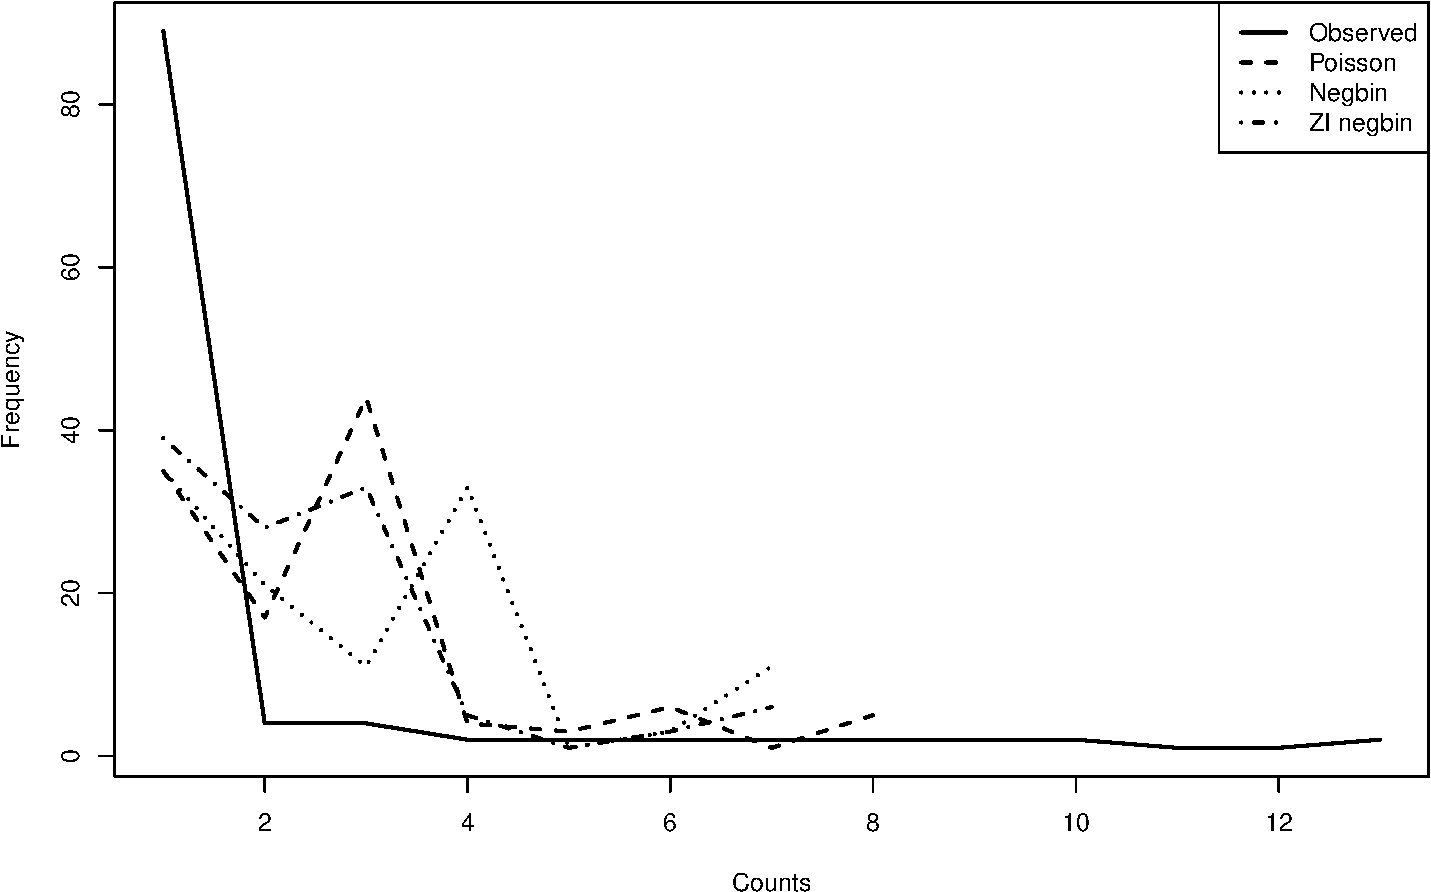
\includegraphics{../docs/articles/session_lecture_files/figure-beamer/unnamed-chunk-24-1.pdf}

\end{frame}

\begin{frame}{Resources for R (and SAS)}
\protect\hypertarget{resources-for-r-and-sas}{}

\begin{itemize}
\tightlist
\item
  Short, practical tutrorials on regression in R and SAS from UCLA at
  \url{http://www.ats.ucla.edu/stat/}:

  \begin{itemize}
  \tightlist
  \item
    Poisson Regression:
    \url{http://www.ats.ucla.edu/stat/r/dae/poissonreg.htm}
  \item
    Negative Binomial:
    \url{http://www.ats.ucla.edu/stat/r/dae/nbreg.htm}
  \item
    Zero-inflated Poisson:
    \url{http://www.ats.ucla.edu/stat/r/dae/zipoisson.htm}
  \item
    Zero-inflated Negative Binomial:
    \url{http://www.ats.ucla.edu/stat/r/dae/zinbreg.htm}
  \end{itemize}
\end{itemize}

\end{frame}

\end{document}
